\documentclass[9pt,twocolumn,twoside,lineno]{pnas-new}
% Use the lineno option to display guide line numbers if required.

\templatetype{pnasresearcharticle} % Choose template 
% {pnasresearcharticle} = Template for a two-column research article
% {pnasmathematics} %= Template for a one-column mathematics article
% {pnasinvited} %= Template for a PNAS invited submission

% macro for citing subfigures
\makeatletter
\newcommand{\phantomlabel}[2]{
    \protected@write\@auxout{}{
        \string\newlabel{#2}{
            {\@currentlabel#1}{\thepage}
            {\@currentlabel#1}{#2}{}
        }
    }
    \hypertarget{#2}{}
}
\makeatother


\title{Interdependent Diffusion: The social contagion of interacting beliefs}

% Use letters for affiliations, numbers to show equal authorship (if applicable) and to indicate the corresponding author
\author[a,b]{James Houghton}
\affil[a]{Massachusetts Institute of Technology}
\affil[b]{University of Pennsylvania}

% Please give the surname of the lead author for the running footer
\leadauthor{Houghton} 

% Please add a significance statement to explain the relevance of your work
\significancestatement{When studying the spread of beliefs from person to person, scholars generally look at only one belief at a time. This paper shows that by focusing on a single belief, we miss interactions between beliefs that lead to polarization. Because polarization is such an important part of why we study social contagion in the first place, recognizing this oversight encourages us to reexamine much of what we know, and opens up a rich sub-field for future research.}

% Please include corresponding author, author contribution and author declaration information
\correspondingauthor{Please direct correspondence to \href{mailto:houghton@mit.edu}{houghton@mit.edu}.\\ See \href{https://github.com/JamesPHoughton/interdependent-diffusion}{https://github.com/JamesPHoughton/interdependent-diffusion} for simulation code, experimental materials, and data. See \href{https://osf.io/239ns}{https://osf.io/239ns} for experiment preregistration.}
%\additionalelement{test}


% At least three keywords are required at submission. Please provide three to five keywords, separated by the pipe symbol.
\keywords{Social Contagion $|$ Social Learning $|$ Simulation $|$ Experiment}  

\begin{abstract}
Social contagion is the process in which people adopt a belief, idea, or practice from a neighbor and pass it along to someone else. For over 100 years, scholars of social contagion have almost exclusively made the same implicit assumption: that only one belief, idea, or practice spreads through the population at a time \cite{granovetter1973strength,burt1992structural,watts1998collective,watts2011simple, reagans2003network,kempe2003maximizing,lazer2007network,travers2011experimental,kearns2006experimental, acemoglu2011opinion,suri2011cooperation,le1897crowd,degroot1974reaching,schelling1978sorting,granovetter1978threshold,centola2007complex,salganik2006experimental,lorenz2011social,muchnik2013social,shalizi2011homophily,golub2012homophily,christakis2013social,rand2011dynamic,almaatouq2020adaptive,galam1991towards,hegselmann2002opinion}. It is a default assumption that we don’t bother to state, let alone justify. The assumption is so ingrained that our literature doesn’t even have a word for “whatever is to be diffused” \cite{granovetter1973strength}, because we have never needed to discuss more than one of them.
But this assumption is obviously false. Millions of beliefs, ideas, and practices (let’s call them ``diffusants'') spread through social contagion every day. To assume that diffusants spread one at a time – or more generously, that they spread independently of one another – is to assume that interactions between diffusants have no influence on adoption patterns. This could be true, or it could be wildly off the mark. We’ve never stopped to find out. 
This paper makes a direct comparison between the spread of independent and interdependent beliefs using simulations, observational data, and a 2400-subject laboratory experiment. I find that in assuming independence between diffusants, scholars have overlooked social processes that fundamentally change the outcomes of social contagion. Interdependence between beliefs generates polarization, irrespective of social network structure, homophily, demographics, politics, or any other commonly cited cause. It also coordinates structures of beliefs that can have both internal justification and social support without any grounding in external truth.
\end{abstract}

\dates{This manuscript was compiled on \today}
%\doi{\url{www.pnas.org/cgi/doi/10.1073/pnas.XXXXXXXXXX}}

\begin{document}

\maketitle
\thispagestyle{firststyle}
\ifthenelse{\boolean{shortarticle}}{\ifthenelse{\boolean{singlecolumn}}{\abscontentformatted}{\abscontent}}{}

% If your first paragraph (i.e. with the \dropcap) contains a list environment (quote, quotation, theorem, definition, enumerate, itemize...), the line after the list may have some extra indentation. If this is the case, add \parshape=0 to the end of the list environment.
\dropcap{O}n June 17\textsuperscript{th}, 2015, the U.S. Treasury announced that a portrait of a woman would appear on the ten-dollar bill \cite{calmes_2015}. The same day, news emerged of a mass shooting at a historically black church in Charleston, South Carolina \cite{houghton2019beyond,hawes2019grace}. Within twenty-four hours both stories had spread throughout U.S. social media. It is reasonable to study the spread of these diffusants independently of one another, because the probability that an individual will share news of the shooting is not likely to be causally influenced by whether they have understood news about the \$10 bill, and vice versa.

The day after the Charleston shooting, two other news items emerged. The first was a report that the shooter had been motivated by racial hatred symbolized in the Confederate flag. The second was a call to remove the Confederate flag from the South Carolina state capitol grounds \cite{houghton2019beyond,hawes2019grace}. Even though these are distinct ideas, each spreading through social contagion, we cannot ignore one in trying to understand the diffusion of the other. If an individual has previously adopted the belief that the flag should be removed from the capitol grounds, they will be more likely to believe that the shooter’s identification with the flag is politically relevant, and vice versa. Rather than being independent diffusants, these beliefs are interdependent. 

With good reason, nearly all social contagion research assumes that diffusants spread independently of one another. The independence assumption makes for parsimonious theory \cite{granovetter1973strength, burt1992structural, watts1998collective, watts2011simple, reagans2003network, kempe2003maximizing, lazer2007network, le1897crowd, degroot1974reaching, schelling1978sorting, granovetter1978threshold, centola2007complex, shalizi2011homophily, golub2012homophily, christakis2013social,galam1991towards,hegselmann2002opinion,acemoglu2011opinion}, and it reduces the complexity and expense of experiments \cite{travers2011experimental, kearns2006experimental, suri2011cooperation, salganik2006experimental, lorenz2011social,muchnik2013social, rand2011dynamic,almaatouq2020adaptive}. The most influential authors on social contagion have used this assumption to study the effect of social network structure \cite{granovetter1973strength,burt1992structural,watts1998collective,watts2011simple, reagans2003network,kempe2003maximizing,lazer2007network,travers2011experimental,kearns2006experimental,suri2011cooperation,acemoglu2011opinion}, social reinforcement \cite{le1897crowd,degroot1974reaching,schelling1978sorting,granovetter1978threshold,centola2007complex,salganik2006experimental,lorenz2011social,muchnik2013social,hegselmann2002opinion}, homophily \cite{shalizi2011homophily,golub2012homophily,christakis2013social}, and network rewiring \cite{christakis2013social,rand2011dynamic,almaatouq2020adaptive} on contagion outcomes. Unfortunately, scholars assume independence between diffusants so frequently and to such productive ends that we generally forget we are doing so, and fail to question whether the assumption is appropriate.

In contrast with independent diffusion, “interdependent diffusion” describes any social contagion process in which individuals’ likelihood of adopting diffusant $A$ is a function of their current state of adoption of $B$ ($C$, $D$, $\ldots$) and in which their likelihood of adopting $B$ ($C$, $D$, $\ldots$) is a function of their state of adoption of $A$. Very few theoretical models include any form of interaction between diffusants \cite{baldassarri2007dynamics,dellaposta2015liberals, friedkin2016network, goldberg2018beyond, xiong2017analysis, axelrod-1997-dissemination}, and none are empirically verified. It remains to be seen whether interdependence between diffusants 1) generates new sociological processes, 2) creates new observable outcomes, and 3) has practical consequences for communication and social policy. In short, does interdependence matter for the theoretical and empirical study of social contagion, or are our models of independent diffusion sufficient?

\section*{Theoretical development}
Interdependent diffusion can be studied through two theoretical lenses. First, we will observe the spread of a ``focal'' belief as it participates in a process of ``reciprocal facilitation'' with other diffusants. Secondly, we will observe a pair of individuals as they exchange multiple beliefs with one another in a process we might call an ``agreement cascade''.

\begin{figure*}[ht]
    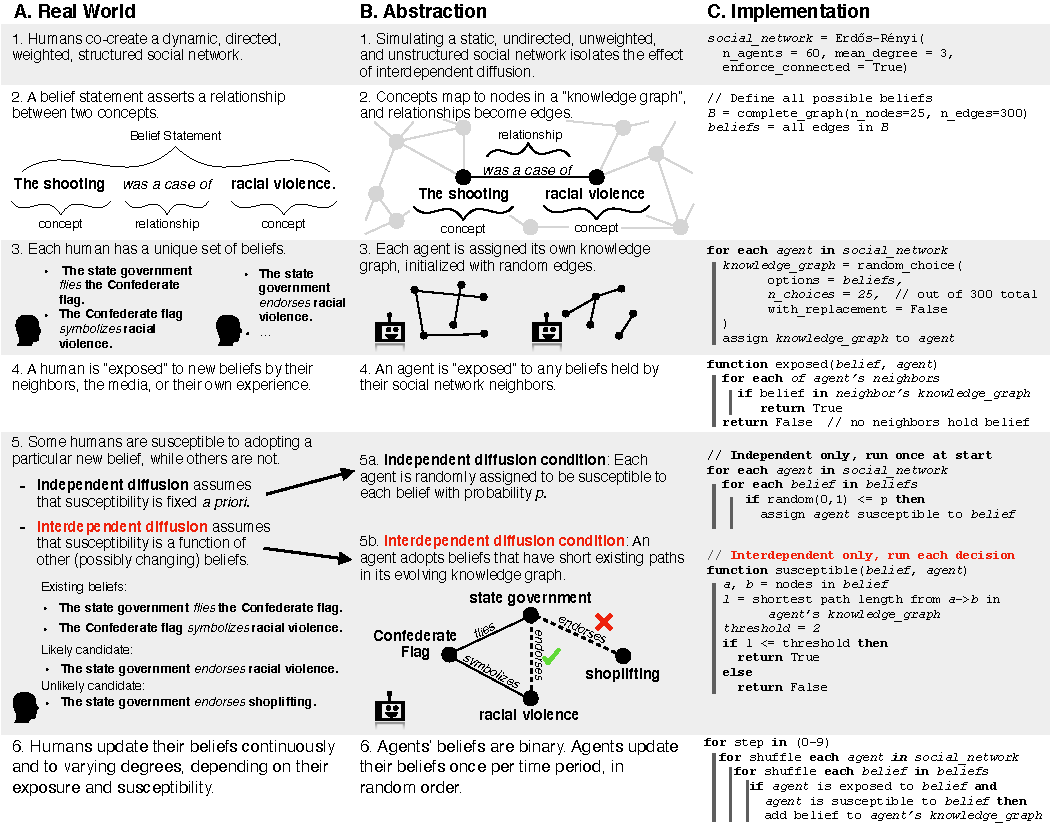
\includegraphics[width=7in]{Fig1.pdf}
    \caption{\textbf{Simulating interdependent diffusion as knowledge graph edges spreading over a social network.} \textbf{A.} In the real world, the effect of interdependence on social contagion is enmeshed with other influences and complexities.  \textbf{B.} A useful abstraction simplifies reality to isolate the mechanisms of interest, and \textbf{C.} allows us to simulate the behavior we wish to understand.}
    \label{fig:model}
\end{figure*}

\subsection*{Reciprocal Facilitation}
A focal belief spreads when an exposed individual’s existing beliefs lead her to think it is true – that is, they ``facilitate'' her adoption of the focal belief. From its new position in the social network, the focal belief may then spread further, and subsequently facilitate the adoption of the beliefs that had previously supported its diffusion. This cycle creates a reinforcing feedback, such that when diffusants alternately create susceptibility to one another they can be adopted by more individuals than any single belief could have reached on its own. We see this ``reciprocal facilitation'' dynamic at work in beliefs about the confederate flag. The existing political conflict facilitated the spread of information about the shooter’s identification with the flag, and as it spread, news of the shooter’s identification with the flag brought more attention to its contentious display at the state capitol. 

We can use a simple agent-based simulation (described in Fig. \ref{fig:model}) to explore the macro-scale effects of reciprocal facilitation. In this simulation, agents populate a fixed, random social network, and are initially assigned a random set of beliefs. Each belief asserts a relationship between two concepts (e.g. \textbf{the shooting} \textit{was a case of} \textbf{racial violence}). By analogy to the ``knowledge graph'' interpretation of semantic networks\cite{sowa1987semantic, collins1975spreading, popping2003knowledge}, an agent's beliefs can be aggregated to form a graph in which nodes represent concepts (e.g. \textbf{people}, \textbf{places}, \textbf{items}, \textbf{activities}, etc\ldots), and edges represent relationships that connect concepts to one another (e.g. \textit{ownership}, \textit{membership}, \textit{co-location}, \textit{usage}, etc\ldots). When an agent adopts a new belief, it becomes a new edge in the agent's knowledge graph.

When an individual is exposed to new beliefs, she prefers to adopt those that connect two concepts that are already close together in her knowledge graph \cite{schilling2005small,nickerson1998confirmation}, as doing so does not require dramatic changes to her belief structure. The simplest representation of this tendency is that a simulated individual will adopt any edge present in at least one neighbor's knowledge graph, as long as the distance it spans in her existing knowledge graph is below some threshold. This decision rule ignores social reinforcement (i.e. no complex contagion) and the exposer's attributes or other beliefs (i.e. no homophily or heterogeneous influence), and so for each belief is equivalent to a simple contagion model in all respects other than the influence of the individual's internal state. Please see the \hyperref[methods]{\textbf{Methods}} section and supplement for details of the simulation and analysis.

Figure \ref{fig:sim1} shows the average results of 20k simulations of 60 agents in the above model. Each agent is assigned random initial beliefs, and adopts beliefs from its social network neighbors that span up to two steps distance in its knowledge graph. First we see that under interdependent diffusion, reciprocal facilitation allows the average number of people susceptible to a belief to grow endogenously with the number of adopters (Fig. \ref{fig:sim1:A}, red). By comparison, if the same beliefs diffuse without interacting (i.e. independently) they can only be adopted by individuals who are susceptible at the start, and so they spread less widely in the population (Fig. \ref{fig:sim1:A}, black). Put another way: to explain the same level of final adoption, models of independent diffusion need to assume significantly more initial susceptibility to each belief. 

\begin{figure}[ht]
    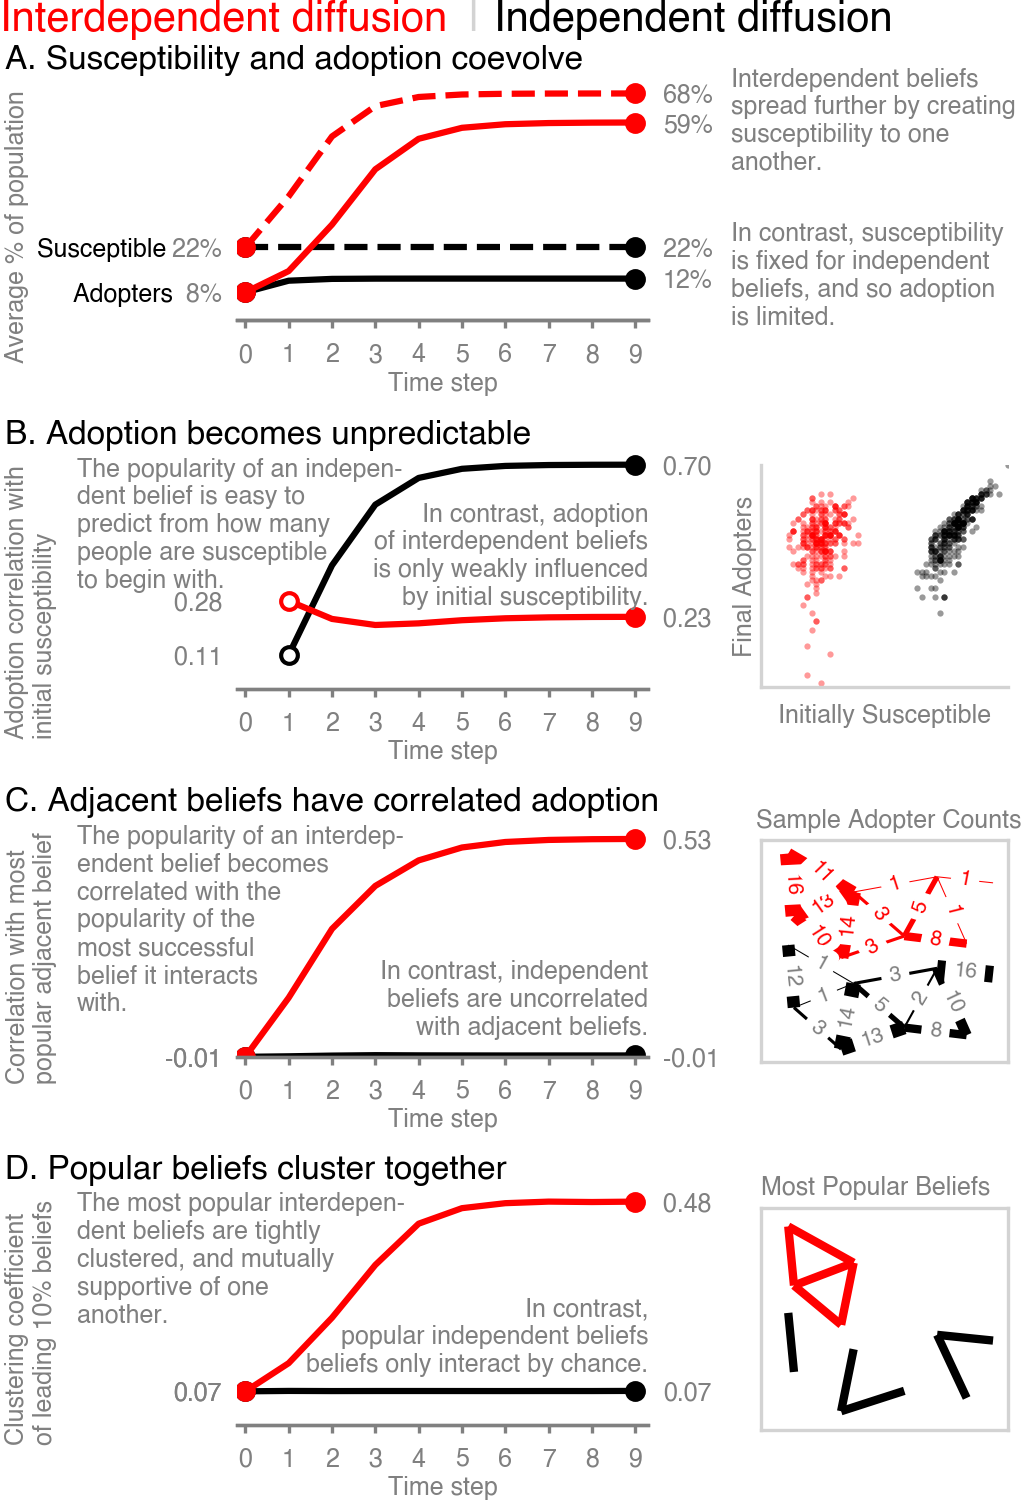
\includegraphics[width=\linewidth]{Fig2_emergent_belief_structures.png}
    \caption{\textbf{Simulated effect of interdependent and independent diffusion on shared belief structures.} \textbf{A.} Average popularity (number of adopters) of all beliefs over time, given an equal number of initially susceptible individuals in each condition. \textbf{B.} Correlation between the initial number of susceptible individuals and the popularity of each belief, given the same \textit{final} distribution of adoption between conditions; detail shows $t=9$ popularity vs. number of individuals initially susceptible. \textbf{C.} Correlation between the popularity of each belief and the popularity of the most popular belief it shares a 'node' with; sample $t=9$ popularity of each belief overlaid on the knowledge graph. \textbf{D.} Clustering coefficient of a hypothetical knowledge graph made up of the most popular 10\% of all beliefs; sample $t=9$ network filtered on popularity.}
    \label{fig:sim1}
    \phantomlabel{A}{fig:sim1:A}
    \phantomlabel{B}{fig:sim1:B}
    \phantomlabel{C}{fig:sim1:C}
    \phantomlabel{D}{fig:sim1:D}
\end{figure}

It might be reasonable for us to ignore interdependence (and instead assume more widespread initial susceptibility) were it not for the second effect of reciprocal facilitation. When diffusants do not interact, the population initially susceptible to a belief is an excellent predictor of who will eventually adopt it (Fig. \ref{fig:sim1:B}). However, when belief are interdependent, individuals can acquire susceptibility by adopting other supporting beliefs, such that initial susceptibility is no longer a strong predictor of eventual adoption. For example, imagine that a “focus group” is selected from our artificial population before the simulation starts, and that amongst this group belief $A$ is adopted by 25\% more people than belief $B$. Unsurprisingly, if we simulate the spread of these beliefs independently of one another, belief $A$ will be more popular than $B$ in over 99\% of cases. On the other hand, when we simulate interdependent diffusion, $A$ is adopted by more people than $B$ only 57\% of the time – just slightly better than chance.

The popularity of interdependent beliefs is hard to predict because the reciprocal facilitation process does not support the diffusion of all beliefs to the same degree. Instead, it preferentially distributes those that are supported by other widely adopted beliefs. Fig. \ref{fig:sim1:C} shows how this reinforcing feedback leads a belief’s popularity to become correlated with that of the most popular belief adjacent to it in the knowledge graph. This is because a belief that is supported by many popular beliefs will have many opportunities to diffuse, and then to facilitate the adoption of other closely related beliefs. Conversely, a belief that is only supported by unpopular beliefs will have trouble reaching even the few individuals who are susceptible to adopting it. 

As a result, patterns emerge when individuals' knowledge graphs are aggregated to the level of the population. After interdependent diffusion, clusters of mutually-supporting beliefs are held by large fractions of the population (Fig. \ref{fig:sim1:D}), and they dictate which new beliefs can be adopted. This is quite remarkable, as \textit{post-hoc}, individuals have both internal support for their beliefs (i.e. each belief is supported by many other beliefs) and external support (i.e. other individuals share both their beliefs and their justifications for believing so). This happens even though \textit{a priori} we have no way to tell which sets of beliefs will become popular, and no ground truth. 

Reciprocal facilitation yields an emergent macro-scale outcome analogous to the micro-scale effect of confirmation bias, in which whole groups of people can collectively deceive themselves through the rational action of comparing new beliefs for consistency with what they already know. This effect doesn't require us to have any prior preference for believing one thing over another, nor does it depend on any in-group vs. out-group sentiment, affinity for similar individuals, network structure, or social reinforcement. It's merely a phenomenon of the social contagion of interdependent beliefs.  

\subsection*{Agreement Cascades}

\begin{figure}[h]
    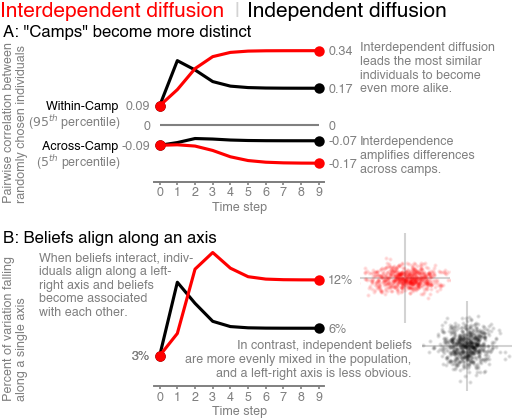
\includegraphics[width=\linewidth]{Fig3_emergent_polarization.png}
    \caption{\textbf{Simulated effect of interdependent and independent diffusion on social polarization.} \textbf{A.} Correlation between beliefs of randomly sampled pairs of individuals, $95^{th}$ ($5^{th}$) percentile represents relationships conservatively within (across) ideological "camps". \textbf{B.} An individual's beliefs locate her in a space with one dimension for each possible belief (300). The percent of variation explained by first principal component of this space describes how well individuals map to a "political spectrum". Offset diagrams are exaggerated and show a larger population to illustrate how a component can explain more or less variation. }
    \label{fig:sim2}
    \phantomlabel{A}{fig:sim2:A}
    \phantomlabel{B}{fig:sim2:B}
\end{figure}

Switching lenses, we now focus on a pair of neighboring individuals, and observe a process of “agreement cascades”. When two people exchange beliefs, they become more similar to one another. Because their existing beliefs influence the way people respond to new diffusants, shared beliefs make the two individuals more likely to adopt (or reject) the same new beliefs in the future. As a result, they become more similar still, regardless of any preference to align or distinguish themselves from one another. 

We can contrast agreement cascades with homophily (i.e. an individual's tendency to give extra weight to the opinions of more similar neighbors \cite{axelrod-1997-dissemination}). When homophily is active, an individual is (consciously or unconsciously) aware of their similarity to a neighbor, and allows that assessment of similarity to influence their adoption decisions. In contrast, agreement cascades increase an individual's likelihood of adopting a belief from a similar neighbor, even if she is blind to every other belief her neighbor possesses. Homophily increases the attractiveness of all beliefs from a similar neighbor, while the same belief shared by a dissimilar neighbor would be less attractive. By contrast, under interdependent diffusion each belief has a particular likelihood of adoption regardless of its source, but agreement cascades mean that similar neighbors provide a higher concentration of beliefs that an individual is likely to adopt. 

Fig. \ref{fig:sim2:A} shows the similarity between pairs of highly similar individuals (whom we might describe as being in the same ``ideological camp'') and highly dissimilar individuals (different camps). Under interdependent diffusion, agreement cascades lead camps to become increasingly self-similar as they expand members’ access to beliefs they can hold in common, and filter out beliefs that would set them apart from one another. Moreover, differences between camps are amplified as existing beliefs drive dissimilar individuals to adopt beliefs from different parts of the belief space.

As individuals organize into camps, it becomes easier to predict each person’s position on one belief from their position on other beliefs. For example, belief $A$ may co-occur with belief $B$ 70\% of the time, but co-occur with belief $C$ only 10\% of the time. This compresses the population’s variation in the space of beliefs into a few principal axes (e.g. liberal-conservative, or libertarian-populist). As a result, differences between individuals can be increasingly described by their position along a “left-right axis”, as seen in Fig. \ref{fig:sim2:B}, with individuals at any point on the axis relatively similar to one another. When beliefs diffuse independently of one another, there is less alignment along the left-right axis and more variation between individuals at any given point. 

\section*{Consistency with observational data}
If reciprocal facilitation and agreement cascades are active in the real world, we should be able to observe the simulation’s predictions in real-world data. For example, when a document asserts a connection between two concepts, then the most popular connections drawn from a corpus of related documents should exhibit more clustering than we expect by chance. Figure \ref{fig:observational:A} shows this effect in article keywords from the New York Times \cite{gallina-etal-2019-kptimes} and academic paper keywords listed in the Web of Science \cite{kowsari2017HDLTex}, over the full range of possible thresholds for a ``popular'' keyword co-occurrence. 

The simulation also predicts that the most similar individuals in the population should be more alike than expected by chance, and those who are dissimilar more different. Figure \ref{fig:observational:B} shows that this prediction is borne out in surveys of political opinions by the Pew Research Center \cite{pew2014} and in surveys of social values by the World Values Survey \cite{wvsa2020}. 

Finally, the simulation predicts that the variation between individuals in these surveys should be more aligned with a few principle axes of polarization than we expect by chance. Figure \ref{fig:observational:C} shows this to be true. Please see the \hyperref[methods]{\textbf{Methods}} section for analysis details.

\begin{figure}[h]
    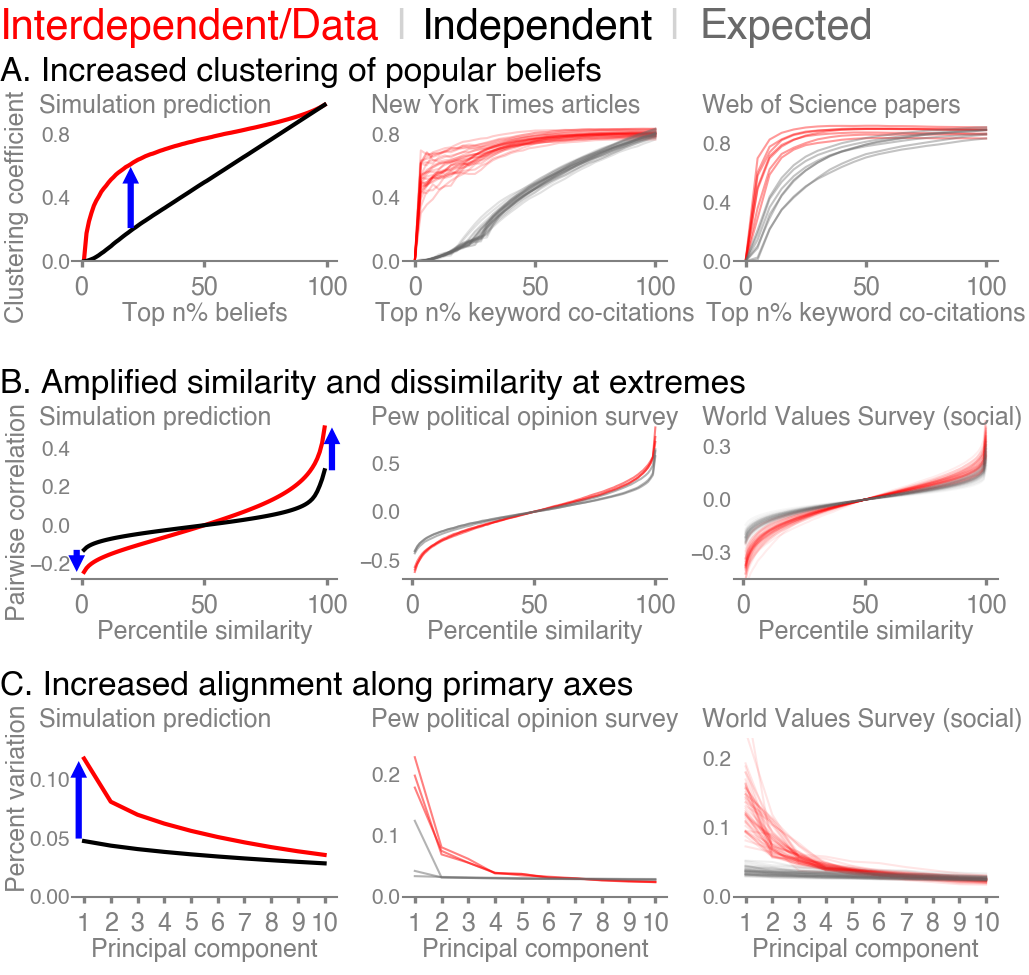
\includegraphics[width=\linewidth]{signatures.png}
    \caption{\textbf{Observing the predicted effects of interdependent diffusion in real-world data.} A. The clustering coefficient of a hypothetical knowledge graph constructed from the $n\%$ most popular beliefs, for $n\in(0,100)$. Interdependence is predicted to increase clustering among the most popular connections between concepts. This increase is observed in keyword co-citation networks from 289k New York Times articles (curves for each of 27 sections)\cite{gallina-etal-2019-kptimes}, and 47k academic papers from Web Of Science (7 fields)\cite{kowsari2017HDLTex}, compared to a randomized baseline.  B. Correlation in beliefs between randomly selected pairs of individuals. Interdependence is predicted to amplify extreme values of similarity and dissimilarity. This amplification is observed among 10k responses to the Pew Political Polarization Survey (3 waves)\cite{pew2014}, and 71k responses to questions about social values in the World Values Survey (49 countries)\cite{wvsa2020}. C. The percentage of variation present in the first 10 components of a principal component analysis. Interdependence is predicted to increase the variance explained by the first few components. This increase is observed in the Pew and World Values surveys.}
    \label{fig:observational}
    \phantomlabel{A}{fig:observational:A}
    \phantomlabel{B}{fig:observational:B}
    \phantomlabel{C}{fig:observational:C}
\end{figure}

\section*{Testing predictions of population-level outcomes in a randomized controlled experiment}
The above simulation describes two mechanisms involved in the social contagion of interacting beliefs, and predicts outcomes that are observed in real world data. However, this model is a simplification of reality, and like all such models may mischaracterize human behavior in important ways. Similarly, observational analysis is limited in this case by the lack of an independent counterfactual; it can only show consistency with the predicted outcomes, rather than causal evidence of the mechanisms themselves. To rigorously test the simulation’s predictions, I conducted a fully preregistered randomized-controlled experiment with 2400 participants. In an online laboratory context, I systematically varied the level of interaction between otherwise identical diffusants in identically constructed populations, and measured macro-scale polarization in behavior and self-reported beliefs. 

To test the macro-scale effect of interdependent diffusion, I designed a ``detective game'' in which participants were given clues to solving a burglary and were asked to sort those clues into ``Promising Leads'' and ``Dead Ends'', using the interface shown in Fig. \ref{fig:game:A}.  When a participant categorized a clue as a promising lead, it was immediately shared with their three neighbors in a 20-person social network, and so could diffuse through the network. Groups played for 8 minutes before reporting their solutions to the mystery. 

In the simulation described in Fig. \ref{fig:model}, agents can be programmed to pay attention to interactions between beliefs in an interdependent condition, and ignore those interactions in an identical independent condition. Human beings, on the other hand, are wired to see connections between ideas, and so it is impossible to conduct a perfect test in which all clues interact in one experimental condition, and yet \textit{the same clues} are fully independent in another. To approximate the ideal manipulation, I partitioned the clues such that some (22 clues) were common to both interdependent and independent conditions and used for analysis (Fig. \ref{fig:game:B}), while the remainder (55 clues) varied across conditions to manipulate the level of interaction between analysis clues. In the interdependent condition, ``cross-link'' clues connected each analysis clue to every other analysis clue (Fig. \ref{fig:game:C}), to create a complete knowledge graph from which players' starting clues could be drawn. In the independent condition, ``filler'' clues gave additional, non-interacting details (Fig. \ref{fig:game:D}) that allowed analysis clues to maintain as much independence as possible. Unknown to participants, clues were designed to equally implicate any suspect or burglary method and were seeded equally in the population. Please see the \hyperref[methods]{\textbf{Methods}} section and the supplement for more details of the experiment.

\begin{figure}[ht]
    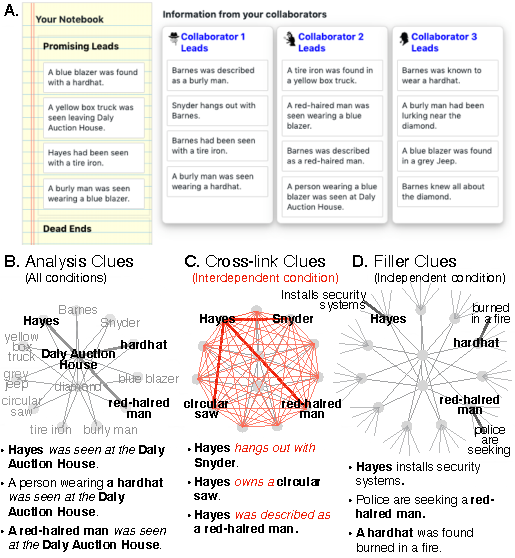
\includegraphics[width=\linewidth]{clues_together.pdf}
    \caption{\textbf{The Detective Game.} \textbf{A.} Player Interface. \textit{``A priceless diamond has been stolen from the Daly Auction House. To solve the mystery, drag clues that you think are true into the ``Promising Leads'' section of your notebook, and clues you think are false into the "Dead Ends" section. You are rewarded for each correct 'lead' and penalized for each incorrect 'lead'. There is no reward or penalty for 'dead ends'.''}
    \textbf{B.} 22 ``analysis'' clues link the crime scene and stolen object to three suspects, two articles of clothing, two descriptions, two tools and two vehicles.
    \textbf{C.} In the interdependent condition, 55 ``cross-link'' clues connect each analysis clue to every other analysis clue.
    \textbf{D.} In the independent condition, ``filler clues'' take the place of cross-link clues, allowing analysis clues to remain independent of one another.
    }
    \label{fig:game}
    \phantomlabel{A}{fig:game:A}
    \phantomlabel{B}{fig:game:B}
    \phantomlabel{C}{fig:game:C}
    \phantomlabel{D}{fig:game:D}
\end{figure}

In a testament to the near-universal pervasiveness of belief interaction, even this manipulation (and ideal laboratory conditions) could not create a control condition with perfectly independent beliefs. For example, even though the independent clue set contained no explicit links between suspects, participants could draw implicit connections between the guilt of one suspect and the presumed innocence of another. This imperfect control means that measured differences between independent and interdependent conditions are likely to underestimate the true effect of belief interaction.

Nevertheless, the results of this experiment support the above macro-level predictions. Figure \ref{fig:experiment:A} shows that among 30 matched pairs of populations, interdependence measurably increased the population’s alignment along a left-right axis among both behavioral (+2.2\% $p=.013$) and self-reported (+2.8\% $p=.022$) measures of belief. While not all measures were significant, camps were more self-similar (behavioral measures +.025 $p=.014$, Fig. \ref{fig:experiment:B}) and more distinct from one another (self-report measures -.035 $p=.058$, Fig. \ref{fig:experiment:C}) in the interdependent condition than in the independent condition.

\subsection*{Comparison effect of social network structure}
To gauge whether the effect of interdependence is large enough to be worth attention when compared to other drivers of polarization, I ran a parallel experimental condition that varied the social network structure between non-polarizing and polarizing extremes. The baseline was a “dodecahedral” network (inset diagram in Fig. \ref{fig:experiment:A}), in which none of a participant’s neighbors were directly connected to any other (network clustering coefficient $0.0$), and the average social network distance between individuals was short ($2.6$ steps). We should expect to find very little polarization in this network, as information can diffuse across the network readily, and coordination among subgroups is impeded by the lack of mutual connections. The second social network was a “regular connected caveman” structure, in which neighbors shared $50\%$ of their remaining contacts in common (clustering coefficient $0.5$), and there are large average distances between individuals ($4$ steps). We should expect to find high levels of polarization in this network regardless of the level of interaction between clues, as strong clustering makes it easy for subgroups to converge on a shared set of clues, and long average path lengths make it harder for information to spread between camps. 

\begin{figure}[ht]
    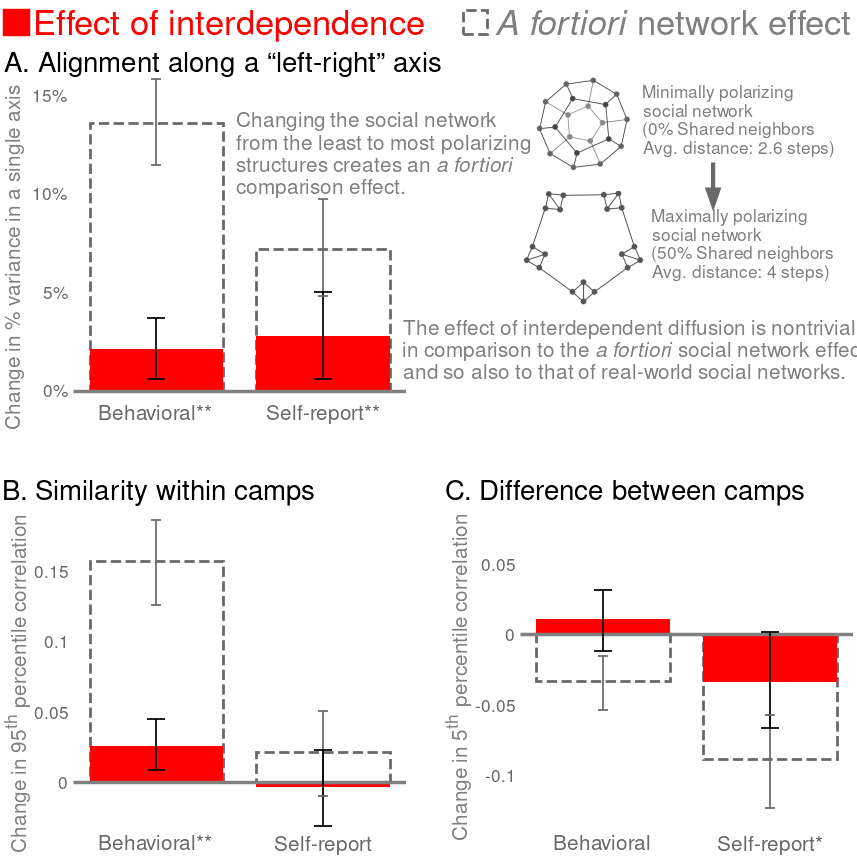
\includegraphics[width=\linewidth]{results_small.png}
    \caption{\textbf{Testing the macro-scale effects of interdependent diffusion in an online lab experiment.} The predicted effects of belief interaction are borne out in experiment, with meaningful effects in comparison to an \textit{a fortiori} comparison. $^*p<.1$, $^{**}p<.05$. Error bars show 90\% CI. $n=30$ pairwise comparisons.}
    \label{fig:experiment}
    \phantomlabel{A}{fig:experiment:A}
    \phantomlabel{B}{fig:experiment:B}
    \phantomlabel{C}{fig:experiment:C}
\end{figure}

Real-world social networks lie somewhere between these two extremes, and so this social network manipulation creates an \textit{a fortiori} comparison effect. If the effect of interdependence is nontrivial in this comparison, then we have confidence that it is meaningful in the real world. In the statistically significant measures of this experiment, interdependent diffusion creates an effect between 16\% and 39\% of the \textit{a fortiori} reference, as shown in Fig. \ref{fig:experiment}. We should always use caution when generalizing effect sizes from laboratory groups to large-scale social networks. However, this comparison suggests that interdependence plays an unignorable role in social contagion, and that scholars’ almost exclusive focus on network structure over belief interaction is out of proportion to the relative importance of the two effects.

\section*{Discussion}
While it cannot explore all of the implications of interdependent diffusion, this paper demonstrates that belief interaction enables at least two new sociological processes that influence polarization and shared belief structures. The social contagion literature is replete with studies that explain polarization as a consequence of social network structure \cite{flache2011small,del2016echo}, homophily \cite{dandekar2013biased,vasconcelos2019consensus,axelrod-1997-dissemination}, complex contagion \cite{spohr2017fake,tornberg2018echo}, or other personal or network characteristics. While they certainly influence polarization, this paper shows that when beliefs interdepend, none of these explanations are necessary for polarization to emerge - polarization is a natural consequence of diffusion itself. Likewise, we have ample research asking how fringe beliefs and conspiracy theories emerge and persist \cite{spohr2017fake,tornberg2018echo,pennycook2019lazy}. Interdependent diffusion suggests that they are a natural consequence of social contagion. 

Given this understanding of interdependent diffusion, we can no longer assume consensus and truth to be the default outcome of social contagion, absent other polarizing factors. No matter what changes we make to the social network structure, or how we reduce interpersonal bias, we should still expect polarization to emerge. This motivates several new research questions: What are the conditions under which populations can overcome the polarizing effect of interdependent diffusion to reach consensus? How can populations avoid deceiving themselves about the truth of the world? Answering these questions will require us to drop the assumption of independence and confront the complex reality of belief interaction in social contagion.

This simulation and experiment remind us that the simplifying assumption of independence between diffusants is just that – an assumption. Despite its ubiquity, the assumption should be carefully made and frequently challenged. With luck we will find that most of what we know about diffusion is robust to interaction between diffusants. We may also find that relaxing the assumption of independence helps us explain new sociological phenomenon and better understand social contagion.

\matmethods{
\label{methods}
All materials used to create this paper (including code for running simulations, observational analysis, designing and conducting the experiment, and analyzing experimental results, along with anonymized, timestamped experimental data) is available at:  \href{https://github.com/JamesPHoughton/detective-game-interdependent-diffusion}{https://github.com/JamesPHoughton/detective-game}. 

\subsection*{Simulation}
In the simulation presented in \textbf{Figs. \ref{fig:sim1} and \ref{fig:sim2}}, the social network is a connected Erdős–Rényi ($G_{nm}$) random graph with 60 agents, each with an average of 3 neighbors. Each agent is initialized with 25 beliefs (edges) selected randomly from the 300 edges available in a complete knowledge graph with 25 concepts (nodes). These values ensure good coverage of beliefs in the population, while individual knowledge graphs are initially sparse. Random seeding ensures that the simulation starts without polarization or systematic variation in belief popularity, and also that the social network structure itself does not contribute to polarization. Because beliefs are drawn from a complete knowledge graph, there is no natural belief structure around which polarization may nucleate. Results are qualitatively similar with other types and sizes of social networks and different sizes and seeding densities of initial knowledge graphs, so long as there are enough beliefs seeded initially for diffusion to occur and not so many that adoption is complete.

In each step, individuals are selected in random order and update their beliefs by incorporating into their knowledge graphs all beliefs (edges) that their neighbors possess and they are susceptible to adopting. In the interdependent case, individuals are susceptible to any belief with an existing path length of 2 (i.e. that closes a triangle) in their knowledge graphs at the current time. In the comparison (independent) case for \textbf{Fig. \ref{fig:sim1:A}}, a random selection of the population is defined to be susceptible to each belief in the same proportion as are initially susceptible to the belief in the interdependent diffusion condition. In \textbf{Figs. \ref{fig:sim1:B}, \ref{fig:sim1:C}, \ref{fig:sim1:D} and \ref{fig:sim2}}, a random selection of susceptible individuals is made in proportion to the final number of susceptible individuals in the interdependent diffusion case. As a result, for all graphs other than \textbf{Fig. \ref{fig:sim1:A}}, a histogram of the extent of diffusion of each belief is approximately the same under both independent and interdependent treatments. This ensures that the subsequent presentation of results reflects purely the effect of interdependence between diffusants, and not the effect of different levels of adoption in the compared populations. Results are qualitatively similar when calculated based upon the initial susceptibility. 

\subsection*{Measures}

In \textbf{Fig. \ref{fig:sim1:A}}, the measure of adopters is the number of individuals with each belief in their knowledge graph, averaged over all beliefs, divided by the total population. Similarly, the measure of the susceptible population (and all discussion of the susceptible population) represents the fraction of individuals who would adopt each belief if exposed to it according to the appropriate decision rule for independent vs. interdependent diffusion, plus the fraction that has already adopted the belief. 
\textbf{Fig. \ref{fig:sim1:B}} shows the Pearson correlation between the number of people who have adopted each belief at time $t$ and the number who were initially susceptible to the belief at $t=0$ but did not start with it. As this has no meaningful value at $t=0$, the curve is drawn from t1-t9.
\textbf{Fig. \ref{fig:sim1:C}} assesses the correlation between the number of individuals who have adopted each belief (knowledge graph edge) and the number who have adopted the most popular belief it shares a 'node' with, averaged over all beliefs. 
\textbf{Fig. \ref{fig:sim1:D}} uses the clustering coefficient of a knowledge graph constructed from the most popular 10\% of beliefs as a demonstration that the most popular beliefs are mutually interrelated, and not merely all related to a single leading belief (e.g. a star or barbell pattern). Clustering only makes sense when beliefs are conceptualized as a knowledge graph. Other conceptualizations of belief interaction might prefer to plot the number of top decile beliefs that each top decile belief interacts with. This measure gives essentially the same result (i.e. large fractional growth over time in the interdependent case, with no change from randomness in the independent case) but fails to capture the mutual inter-relatedness indicated by the clustering coefficient. The measure is generally insensitive to the specific threshold used to define a ‘popular’ belief for any thresholds between about 5\% and 40\%. See the supplement for sensitivity analysis. 

There are many complex measures of polarization in the literature \cite[for a sample]{baldassarri2007dynamics,dellaposta2015liberals,goldberg2018beyond,flache2011small,del2016echo,dandekar2013biased,vasconcelos2019consensus,spohr2017fake,tornberg2018echo,pennycook2019lazy}, which generally attempt to represent three basic intuitions. First, that individuals within the same ideological camp come to be more similar to one another. Secondly, that individuals in different ideological camps become more dissimilar to one another. Lastly, that an individual’s position on one dimension of belief becomes informative of their position on other dimensions. As my purpose is not to identify camps and their members, but to suggest that one set of conditions is more generative of polarization than another, these measures add more complexity than value. Instead I report heuristic measures characterizing the above three intuitions.

A simple and reproducible way to assess the similarity of individuals within an ideological camp – absent exogenous labels such as demographic or party – is to measure the similarity between all pairs of individuals and define a certain percentile as belonging to the same ideological camp. The more exclusive we are (i.e. the higher the percentile), the more conservative the claim that these represent “within-camp” relationships. To define across-camp similarity, we can choose a percentile that (conservatively) represents relationships between individuals in different ideological camps. In \textbf{Figs. \ref{fig:sim2:A}, \ref{fig:experiment:B}, and \ref{fig:experiment:C}}, I use the $95^{th}$ and $5^{th}$ percentiles respectively. See the supplement for sensitivity analysis.

\textbf{Figs. \ref{fig:sim2:B}, \ref{fig:observational:C} and \ref{fig:experiment:A}} measure belief alignment as the percent of variation between individuals that can be explained by the best fitting axis in the space of possible beliefs, using singular-value decomposition. In \textbf{Fig. \ref{fig:sim2:B}}, the original feature space has one dimension for each belief in the simulation (300), and points representing each individual’s position in that feature space (60) according to the beliefs they have adopted. The offset graphs are exaggerated and show a larger population to illustrate how a component can explain more or less variation. In \textbf{Fig. \ref{fig:experiment:A}}, the feature space has 22 dimensions for the behavioral measures, and 11 dimensions for self-report measures (described below), and points representing 20 individuals.

\subsection*{Analysis of observational data}
The first column in \textbf{Fig. \ref{fig:observational}} shows simulated measures of belief clustering, inter-subject similarity, and percent variance in a given principal component over a range of thresholds and principal components, using the same simulation parameters described previously. 

In order to assess clustering of popular beliefs in \textbf{Fig. \ref{fig:observational:A}}, a dataset needs to include a large diversity of connections between concepts. New York Times article data is taken from the KPTimes dataset\cite{gallina2019kptimes}, including 13 years of articles for all categories with $>= 3000$ documents. One line is shown for each of 27 news sections, each computed independently. When multiple categories were indicated, a document was assigned to the smallest category with $>= 3000$ documents. A weighted undirected graph was constructed for each category, in which article keywords formed nodes, and edges were weighted by the number of articles tagged with the two keywords in the edge. An alternative method in which edges are constructed by random draws without replacement gives the same qualitative effect, and is detailed in the supplement. Data on Web of Science paper keywords\cite{kowsari2017HDLTex} used the same analysis, showing one line for each of 7 major academic fields. 

In order to assess similarity and political axis alignment in \textbf{Figs. \ref{fig:observational:B} and \ref{fig:observational:C}}, a dataset needs dense information about individual beliefs. Political opinion data comes from 58 political opinion questions from the Pew Political Typology Survey\cite{pew2014}, conducted in three waves in early 2014.
The social values analysis uses 144 questions regarding non-political social values in the World Values Survey\cite{wvsa2020} collected from 2017-2020. Missing, unknown, and refused responses ($<5\%$) are filled with the mean values for each question for each wave or country. As in the simulations above, similarity between individuals is assessed as the Pearson correlation of their responses to survey questions. Similarity curves are median-shifted in order to cleanly show the effect on all waves in the same plot. Principal components are computed from a space initially consisting of one dimension for each survey question. A full list of survey questions used is available in the supplement.

As we have no counterfactual world in which diffusion is assuredly independent, I compare the observed data to a synthetic control generated by shuffling beliefs among documents or individuals.

\subsection*{Experiment}
The preregistration for this experiment included all code necessary to conduct the experiment using Empirica\cite{almaatouq2021empirica} and perform all statistical analyses reported in this paper. No analysis decisions were made after preregistration. The preregistration is available at \href{https://osf.io/239ns}{https://osf.io/239ns}.

Over the course of eight days in July 2020, I recruited 2768 U.S. and Canadian Mechanical Turk workers under the criteria that they were 18+ years old, and have completed 100+ HITs with a 90\%+ approval rating. Of these, 2400 completed training and were randomized into 20-person social networks. Each network was assigned to one of four (matched) experimental conditions, yielding $n=30$ samples per condition. This sample size was set by budget constraints. The participant population was 45\% female; mean 37.1 years old; 27\% high-school, 49\% bachelors, 16\% masters+ graduates. 96.8\% of players who completed training went on to complete all steps of the experiment, with less than 0.4\% difference in dropout between conditions. 
%Participants were paid \$0.10 for showing up, \$1 for training in how to use the interface, \$1 to participate, up to \$1 individual performance bonus, and up to \$1 for the performance of their team. 
The average payout was just over \$4, and the experiment took about 20 minutes. 

Clues were extensively pre-tested to minimize bias from the outside world, such that each element was perceived to be equally likely to be involved in a burglary absent other information. Sets of clues were then randomly generated from the pool of pretested elements, representing over 225 billion possible mysteries. At the start of the game, each clue was present in exactly one player’s notebook. As a result, beliefs spread on a level playing field, such that \textit{a priori} none should be expected to diffuse more than any other.  

Together, the clue structure and social network manipulations create four separate conditions. The dodecahedral network and independent clue set formed a baseline condition. Contrasted with the baseline, experimental conditions measured the effect of interdependence, the effect of social network structure, and the effect of both manipulations combined. Blocks of four simultaneous games were constructed with one game in each condition. To guard against latent external biases, each block used a different randomly-generated set of clues. Clue assignments varied as little as possible within each block, such that the clues assigned to a particular network position in one game corresponded to those assigned to the same network position in the other three games. Upon completing training, participants were randomly assigned to positions within a block, blind to their treatment condition. I treated games within each block as matched samples. As there is a strong theoretical prior for the direction of each effect, I used one-sided pairwise t-tests to assess the differences between each experimental condition and the baseline. 
%Bootstrapped confidence intervals in Fig. \ref{fig:experiment} include $90\%$ of resampled cases, to correspond with the one-sided pairwise t-tests at $p<.05$ level.

The measures of polarization described in the above simulation were operationalized to reflect participants’ behavior, and also their self-reported opinions.  ``Behavioral'' measures were constructed from each participant’s final categorization of the 22 analysis clues (i.e. the clues that were common to both the independent and interdependent condition), reflecting the cumulative choices that the participants had made throughout the game. Following the game, participants estimated the likelihood that each suspect, vehicle, etc. was involved in the crime. “Self-report” measures were constructed from these 11-item assessments, reflecting how participants internalized the information they encountered to create opinions. Finally, participants were asked to rate their confidence in their overall solution, and the level of consensus they perceived in their team. 

Similarity between self-reported measures is assessed using Pearson’s correlation on the vectors of individuals’ responses. This measure has the advantage of being easily interpretable and having a well-defined range that is independent of the number of features in the vector of attributes being compared, and the negative region of which can be interpreted as expressing dissimilarity. To assess the similarity of the binary “behavioral” data I use the Phi coefficient, an analogous measure to Pearson’s correlation with the same interpretable range.

The behavioral measures in the experiment are sensitive not only to interdependence and network structure but also to the average level of diffusion of beliefs. To minimize noise due to differences in the level of activity between games, each of the behavioral measures is assessed compared to what would be expected due to chance, keeping the number of adopters of each clue and the number of clues adopted by each participant fixed. This correction was designed in simulation and preregistered.

Additional details and outcomes of secondary analyses are reported in the supplement.
}

\showmatmethods{} % Display the Materials and Methods


% \subsection*{Author Affiliations}
% Include department, institution, and complete address, with the ZIP/postal code, for each author. Use lower case letters to match authors with institutions, as shown in the example. PNAS strongly encourages authors to supply an \href{https://orcid.org/}{ORCID identifier} for each author. Individual authors must link their ORCID account to their PNAS account at \href{http://www.pnascentral.org/}{www.pnascentral.org}. For proper authentication, authors must provide their ORCID at submission and are not permitted to add ORCIDs on proofs.

% \subsection*{Format}
% Many authors find it useful to organize their manuscripts with the following order of sections;  title, author line and affiliations, keywords, abstract, significance statement, introduction, results, discussion, materials and methods, acknowledgments, and references. Other orders and headings are permitted.

% \subsection*{Manuscript Length}
% A standard 6-page article is approximately 4,000 words, 50 references, and 4 medium-size graphical elements (i.e., figures and tables). The preferred length of articles remains at 6 pages, but PNAS will allow articles up to a maximum of 12 pages.


% \subsection*{Digital Figures}
% EPS, high-resolution PDF, and PowerPoint are preferred formats for figures that will be used in the main manuscript. Authors may submit PRC or U3D files for 3D images; these must be accompanied by 2D representations in TIFF, EPS, or high-resolution PDF format. Color images must be in RGB (red, green, blue) mode. Include the font files for any text.



% \subsection*{Supporting Information Appendix (SI)}
% Authors should submit SI as a single separate SI Appendix PDF file, combining all text, figures, tables, movie legends, and SI references. SI will be published as provided by the authors; it will not be edited or composed. Additional details can be found in the \href{https://www.pnas.org/authors/submitting-your-manuscript#manuscript-formatting-guidelines}{PNAS Author Center}. The PNAS Overleaf SI template can be found \href{https://www.overleaf.com/latex/templates/pnas-template-for-supplementary-information/wqfsfqwyjtsd}{here}. Refer to the SI Appendix in the manuscript at an appropriate point in the text. Number supporting figures and tables starting with S1, S2, etc.

% Authors who place detailed materials and methods in an SI Appendix must provide sufficient detail in the main text methods to enable a reader to follow the logic of the procedures and results and also must reference the SI methods. If a paper is fundamentally a study of a new method or technique, then the methods must be described completely in the main text.






\acknow{Special thanks to Abdullah Almaatouq, Sinan Aral, Carolyn Fu, Hazhir Rahmandad, David Rand, Ray Reagans, Hagay Volvovsky, Duncan Watts, and the System Dynamics and Economic Sociology groups at MIT Sloan for their guidance. }

\showacknow{} % Display the acknowledgments section

% Bibliography
\bibliography{references}

\end{document}
